\clearpage
\section{Costs}
\label{app:costs}

\paragraph{Inference at common token prices.}
Figure~\ref{fig:inference-cost} reprices the stream tokens of Figure~\ref{fig:plane}'s learners at the same tariff per model (Table~\ref{tab:inference-pricing}). For QDE this is an API-equivalent serving cost, not its GPU bill or a claim that the provider hosts its adapters. QT, QTE and QETE include the teacher's online play; QDE excludes training compute and teacher labels. Costs are divided by all users' valid stream instances and exclude the reset runs and final tests.

Per-run resource records do not retain cache-hit counts. We therefore assume 70\% cached input for both models and show the full sensitivity to that fraction, from 0 to 100\%. These are serving scenarios, not measured bills. Output counts already include reasoning tokens.

\begin{table}[htbp]
\centering
\footnotesize
\begin{tabular}{llrrr}
\toprule
Model & Provider & Input & Cached input & Output \\
\midrule
Qwen3.5-9B & PrimeIntellect & 0.020 & 0.018 & 0.030 \\
GLM-5.3-Flash & Z.ai & 0.150 & 0.030 & 0.500 \\
\bottomrule
\end{tabular}

\caption{US dollars per million tokens, retrieved on 7 November 2026. Qwen uses PrimeIntellect's BF16 endpoint on \href{https://openrouter.ai/api/v1/models/qwen/qwen3.5-9b/endpoints}{OpenRouter}; GLM uses \href{https://docs.z.ai/guides/overview/pricing}{Z.ai}.}
\label{tab:inference-pricing}
\end{table}

\begin{figure}[htbp]
\centering
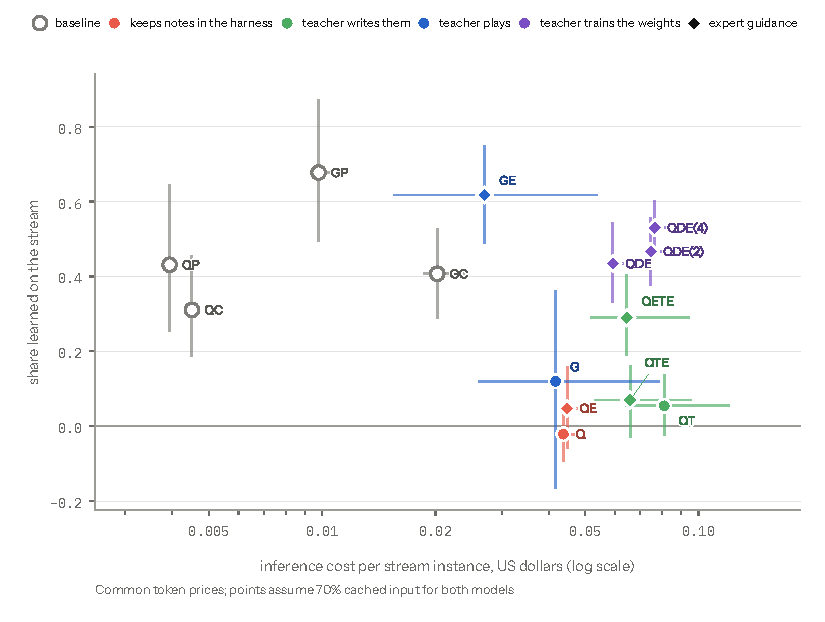
\includegraphics[width=\linewidth]{figures/inference-cost.pdf}
\caption{Inference cost and share learned on the stream, with labels as in Figure~\ref{fig:plane}. Vertical bars are pointwise 95\% task-bootstrap intervals; horizontal bars span 0 to 100\% cached input, with points at 70\%. QDE(2) and QDE(4) serve two and four users; every other learner serves one.}
\label{fig:inference-cost}
\end{figure}

\clearpage
\paragraph{Recorded experiment spending.}
Table~\ref{tab:experiment-costs} sums the recorded API charges for the final run families, their controls and test repeats, the Luna order comparisons, and the reported calibrations. Shared controls and teacher streams are counted once. The training estimate uses completed phase durations and GPU allocations, with corrections when a resumed phase changed allocation, at \$4.50 per H100-hour.

The API subtotal is incomplete: some provider charges and failed teacher-label calls were not recorded. GPU serving, idle allocation, earlier configuration searches and failed methods are also excluded. These figures therefore give a documented portion of the experiment costs, not the project's total bill. The released cost manifest lists every included source and the exclusions.

\begin{table}[htbp]
\centering
\footnotesize
\setlength{\tabcolsep}{4pt}
\begin{adjustbox}{max width=\linewidth}
\begin{tabular}{lrrr}
\toprule
Experiment group & Recorded API (\$) & H100 hours & Est. training (\$) \\
\midrule
ARC-AGI-1, Qwen and GLM & 5,735.66 & -- & -- \\
ARC-AGI-1, Luna (three efforts and orders) & 4,406.10 & -- & -- \\
ARC-AGI-2, Kimi methods & 898.03 & -- & -- \\
ARC-AGI-3, Kimi methods & 698.62 & -- & -- \\
Private-set and ARC-AGI-2 calibration & 83.18 & -- & -- \\
QDE, 1 user: labels and training & 70.81 & 262.8 & 1,182 \\
QDE, 2 users: labels and training & 170.33 & 293.3 & 1,320 \\
QDE, 4 users: labels and training & 344.00 & 368.4 & 1,658 \\
\midrule
Subtotal & 12,406.75 & 924.5 & 4,160 \\
\bottomrule
\end{tabular}

\end{adjustbox}
\caption{Recorded API charges and estimated H100 training costs, in US dollars. QDE's rows give its teacher-label charges and training over all completed phases of its one-, two- and four-user runs.}
\label{tab:experiment-costs}
\end{table}
